% author_page.tex (simplified: whole page is a single screenshot image)
%
% This file is \input inside the preamble (before \begin{document}), so it
% must only DEFINE the \MakeAuthorPage command here -- it must not typeset
% anything directly. The actual page is drawn later, in the body, at the
% point where whitepaper_book.tex calls \MakeAuthorPage.
%
% Note: \includegraphics is used directly (NOT inside a \begin{figure}...
% \end{figure} float). A "figure" is a floating environment, so LaTeX is
% free to push it to a different page if it doesn't fit -- that is why the
% author page could end up somewhere other than right after the cover.
% Placing \includegraphics directly guarantees it stays exactly where
% \MakeAuthorPage is called.
 
\newcommand{\MakeAuthorPage}{%
  \clearpage
  \thispagestyle{empty}
  \begin{center}
    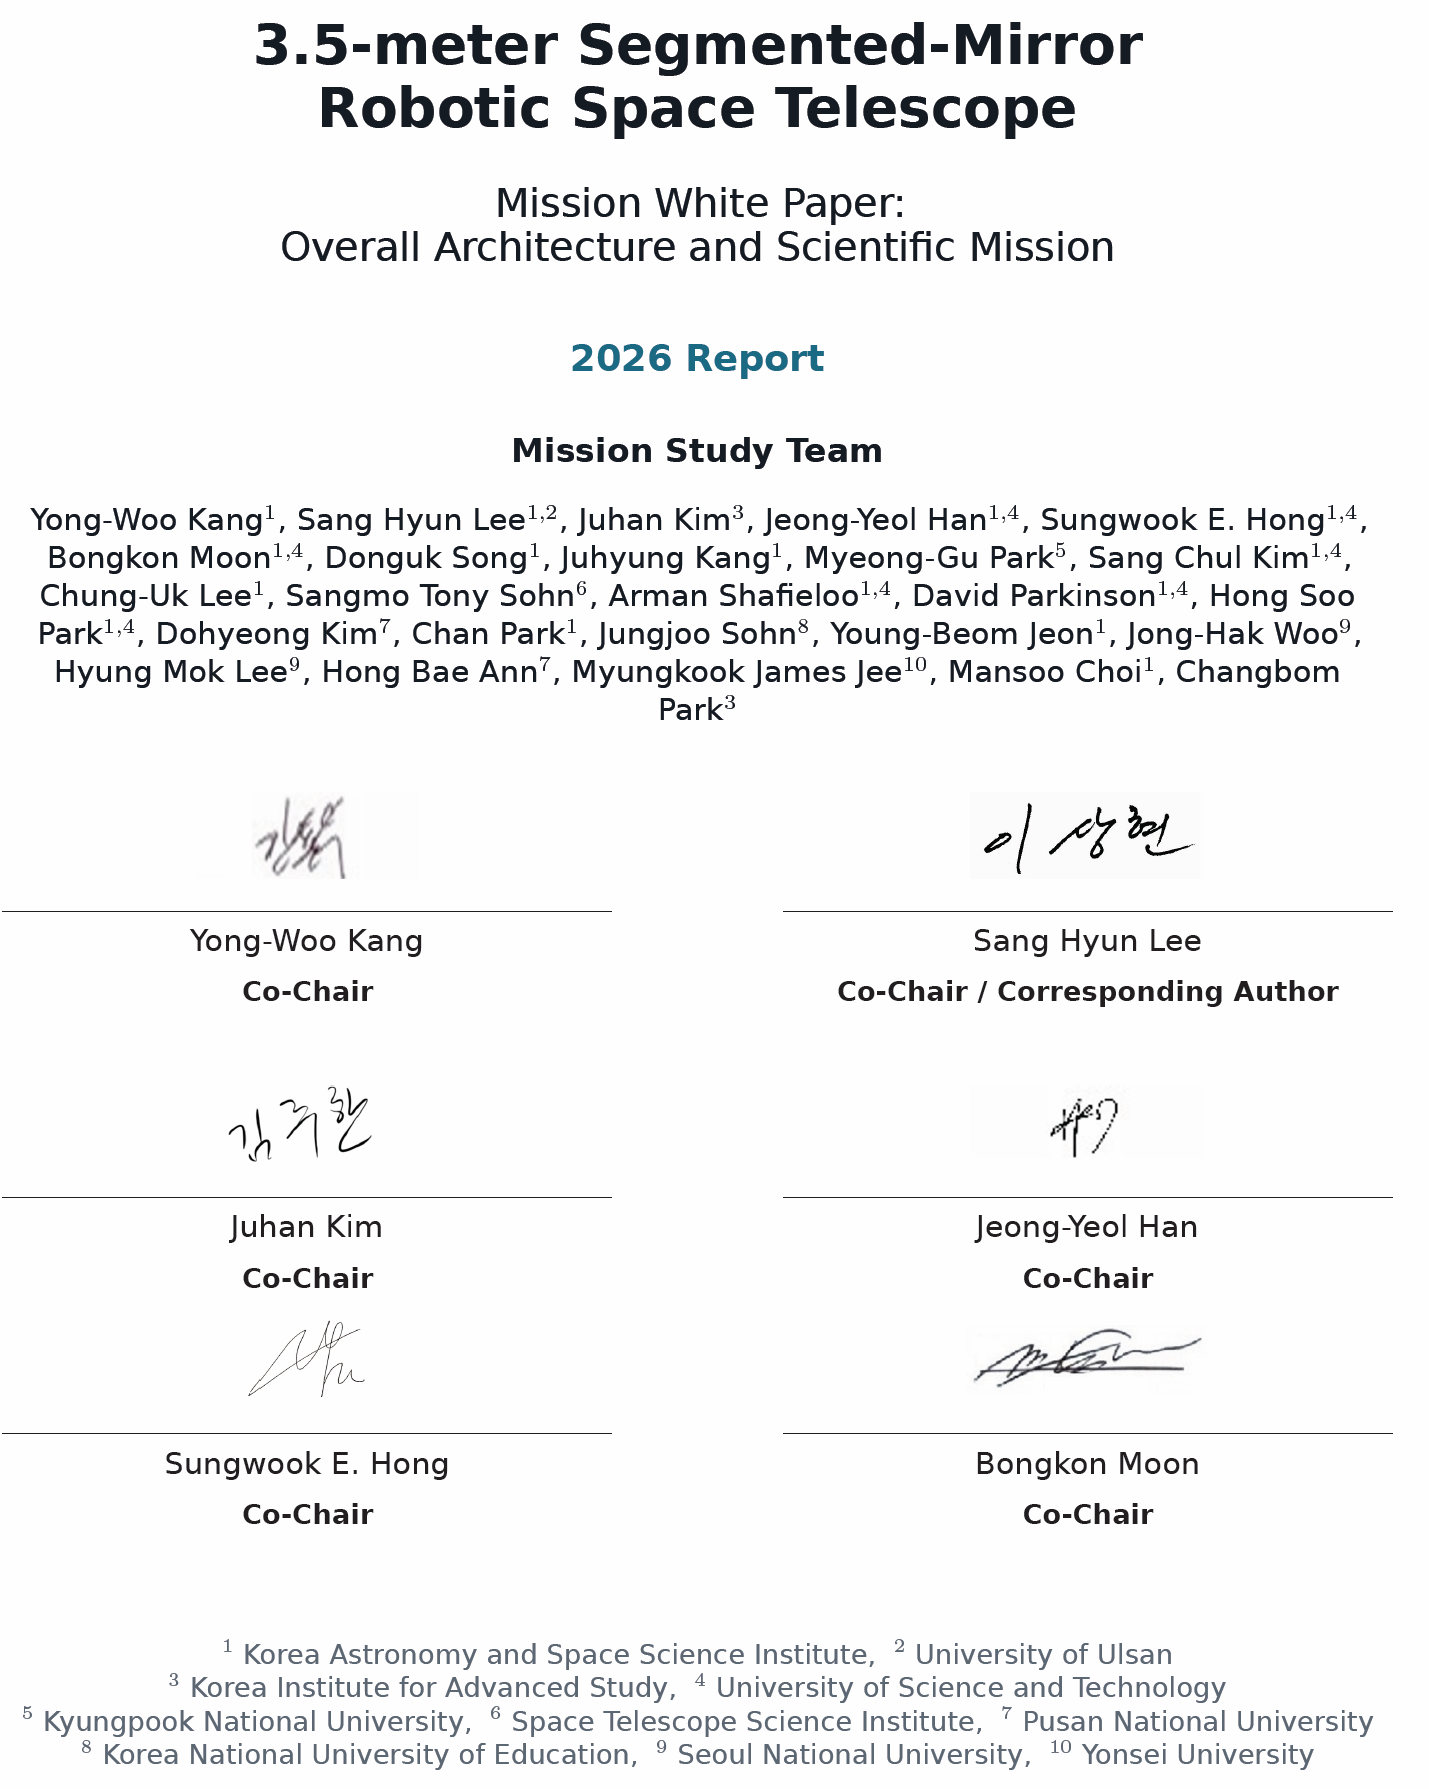
\includegraphics[width=\textwidth,height=0.95\textheight,keepaspectratio]{vol1_author.png}
  \end{center}
  \clearpage
}
 
